\chapter{Simulation Software}
\label{ch:xoopic}


The PIC simulation program used in this project is called \textit{X11 object-oriented particle-in-cell} (XOOPIC). It is a C/C++ based program that simulates 2D plasma systems. It was originally developed in the 1990s by the Plasma Theory and Simulation Group from the University of California at Berkley \cite{Verboncoeur1995}. The code base was subsequently forked by the Plasma and Pulsed Power Group at Loughborough University, and improved upon to include additional features and output diagnostics for analysis.


\section{Overview}

XOOPIC is primarily a command-line-interface (CLI) program but support X11 windowing to visualise certain diagnostics in real time. Some examples of these real time diagnostics include: average kinetic energies of the particles, phase-space plots of the position and velocities of the various particle species,
and the electric field vectors at the simulation grid. While important for determining the behaviour of the plasma system, running the simulation with these windows does significantly reduce its performance. Therefore, XOOPIC's in-built visualisations are primarily used to observe the snapshot behaviour of the simulated system, whilst any diagnostic information required for further analysis is typically written into output files.

Despite not running with X11 windowing, running these simulations continuously takes a long period of time (typically on the order of days to weeks) before they settle into a steady state. This is because the simulations have to be run at very small time steps in order to be stable (see section 4.1.2). 

\subsection{Remote Server}

Due to this long simulation time, running XOOPIC simulations continuously on a local machine are just not feasible. Instead, simulations are run remotely on Loughborough University's high performance servers via \textit{secure shell} (SSH). Typically, multiple simulations are run concurrently in order to test various model parameters.

There are several risks associated with running simulations using a remote server. The first being that if (and when) the connection between the client and the server is severed, the simulations will be killed by the server. This problem can be alleviated with the use of terminal multiplexors, such as \textit{GNU Screen}\footnote{https://www.gnu.org/software/screen/}. This allows for the creation of multiple pseudo-terminal sessions that run in the background. Once created, the client is free to attach and detach sessions without the need for an uninterrupted connection to the server. 

A broken client-server connection is not the only way a simulation can be terminated. Some others include unexpected server restarts, power outages, or overuse of server resources due to memory leaks. In such cases, the simulation can be resumed using XOOPIC's dump files (also referred to as restart files). These files are essentially periodic saves of the simulations and can be used to restart the simulation from the last save point if the need arises. The save interval between dump files is set when starting the simulation. Though tempting to set this interval as small as possible in order to mitigate any data loss, generating these files is very expensive computationally as it involves writing most of the simulation variables onto disk. Thus, the dump file interval are set in the neighbourhood of hundreds of thousands of time steps. 

\subsection{Input Files}

The parameters for XOOPIC's simulations are set using an input file. This is simply a custom formatted text file, with a pseudo-JSON-like structure. The input file is divided into three sections: headers, variables, and region. The first two sections are for the user's benefit, describing the simulation and the parameter values used respectively. 

The region section however is where the true simulation parameters are specified. It can be further sub-divided into multiple subsections. The list of all possible subsections is vast, though a typical PIC simulation includes:

\begin{itemize}
	\item \textbf{Grid} where the dimensions of the plasma device are specified, either in cylindrical or cartesian geometry.
	\item \textbf{Control} where the control parameters such as the size of the time step or a flag to use a specific field solver are set.
	\item \textbf{Species} which state parameters of the particle species being simulated, for example its mass and charge.
	\item \textbf{MCC} that determine the collision characteristics of the plasma based on the background gas pressure and temperature. The collisions can also be turned off outright.
	\item \textbf{Load} that establishes the region in which the particle species are loaded.
	\item \textbf{Diagnostic} which as the name suggests extracts the various diagnostic information and saves them to an output file.
\end{itemize}

The other subsections not listed are the various boundary parameters. The usage of these parameters will vary based on the type of device being simulated. Some examples of      boundary parameters include: a grounded boundary, a current source, and a dielectric boundary. 

When constructing the input files, care must be taken to ensure that the grid size (within the grid subsection) and the time step (within the control subsection) obey a set of conditions so that the simulation is stable. 

The grid size of the simulation, $\Delta x$ and $\Delta y$ should adhere to the equation \cite{Hockney1988}:
\begin{equation}
	\Delta x < 3.4 \lambda_{D}
\end{equation}
where $\lambda_D$ is the Debye length. This is to ensure that the electric fields in the sheath can be resolved.

As for the time step, $\Delta t$, it should be able to resolve the plasma oscillations, thus should satisfy the equation \cite{tskhakaya_matyash_schneider_taccogna_2007}:
\begin{equation}
	\Delta t < 0.2 \omega_{pe}^{-1}
\end{equation}
where $\omega_{pe}$ is the plasma frequency. Note, this condition is only valid for electrostatic plasma simulations. 


\section{Improvements}

During the course of this project, several improvements were made to XOOPIC. This primarily included bug fixes, but also the inclusion of a new boundary parameter (within the region section) called the \textit{Circuit} boundary. 

\subsection{Motivation}

XOOPIC previously had two types of (traditional) input source boundaries. An ideal voltage source, known as the \textit{Equipotential} boundary; and an ideal current source, called the \textit{Current Source} boundary. 

With the Equipotential boundary, the simulation always keeps the potential at the boundary equal to the source voltage specified in the input file. This has the issue where there are no maximum or minimum bounds for current though the boundary. Thus, theoretically the current though the boundary can grow exponentially to infinity. In practice however, the simulation simply becomes unstable and crashes. It is also possible for this current to exceed the rated current of the intended power supply to be used.

Likewise with the Current Source boundary, the simulation attempts to keep the current across the boundary at a constant specified value; despite the potential at the boundary. And in practice, it is possible that the potential produced by the simulation exceeds the voltage that can be delivered by the power supply. 

Hence, in order to accurately simulate a ``real world" power supply, the Circuit boundary was introduced. This boundary represents the configuration of an ideal voltage source with a resistor attached in series. An illustration of this can be seen in figure \ref{fig:circuit}. The one significant assumption with this boundary is that the circuit shares the same ground plane as the rest of the plasma device being simulated, which is normally the case. 

\begin{figure}[h!]
	\centering
	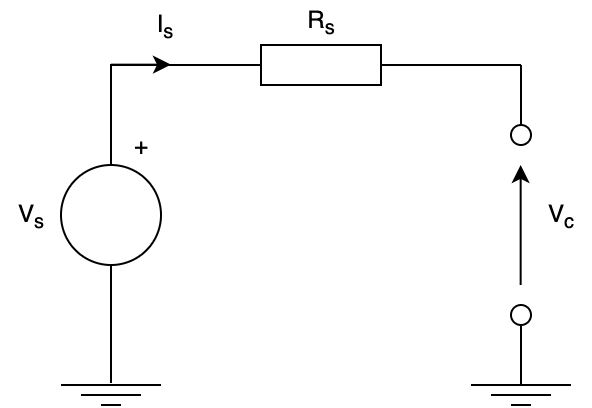
\includegraphics[width=0.59\linewidth]{xoopic/figures/circuit.png}
	\caption{Illustration of circuit boundary.}
	\label{fig:circuit}
\end{figure} 

By adding the series resistor, in effect the maximum voltage and current across the boundary has been limited. As seen in figure \ref{fig:circuit_vi_graph}, the maximum voltage is obtained when the simulated device is an open circuit. As for the maximum current, it is achieved when the simulated device behaves as a short circuit. Thus the potential of the Circuit boundary can be given by:
\begin{equation}
	V_c = V_s - I_s R_s	
	\label{eq:circuit_equation}
\end{equation}

\begin{figure}[h!]
	\centering
	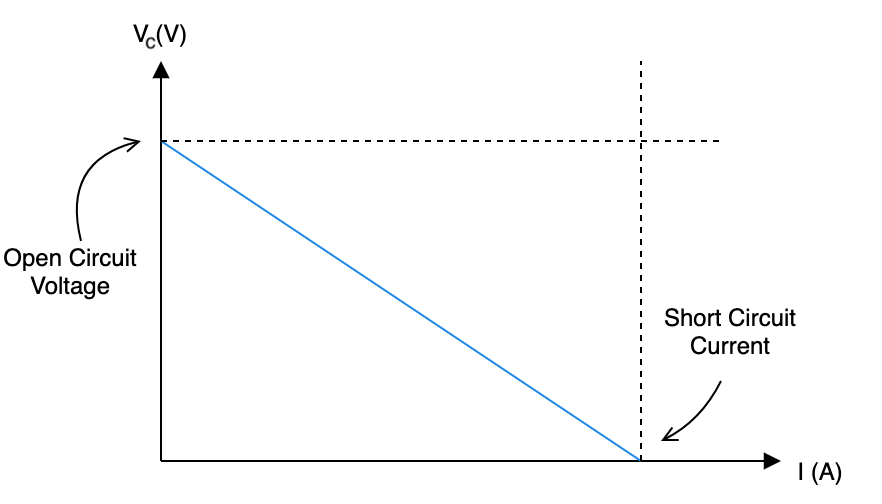
\includegraphics[width=0.8\linewidth]{xoopic/figures/circuit_vi_graph.png}
	\caption{Voltage-current relationship of circuit boundary.}
	\label{fig:circuit_vi_graph}
\end{figure} 

\subsection{Methodology}

As mentioned previously, XOOPIC has the capability of performing simulations in cartesian geometry or cylindrical geometry. Hence an implementation was required for both geometry types. For this report, a general solution based on \cite{Verboncoeur1993, Vahedi1997} is first described, followed by the specific coefficient values required in either geometry.

\subsubsection{General Solution}

A case for the Circuit boundary shown in figure \ref{fig:circuit_general_case}. The points represent an arbitrary fixed grid, with grid points labelled $i$ and $j$ that correspond to the relative positions along the horizontal and vertical directions respectively. The boundary itself is represented by the vertical line, placed along the left most grid points, where $i=0$. 

\begin{figure}[h!]
	\centering
	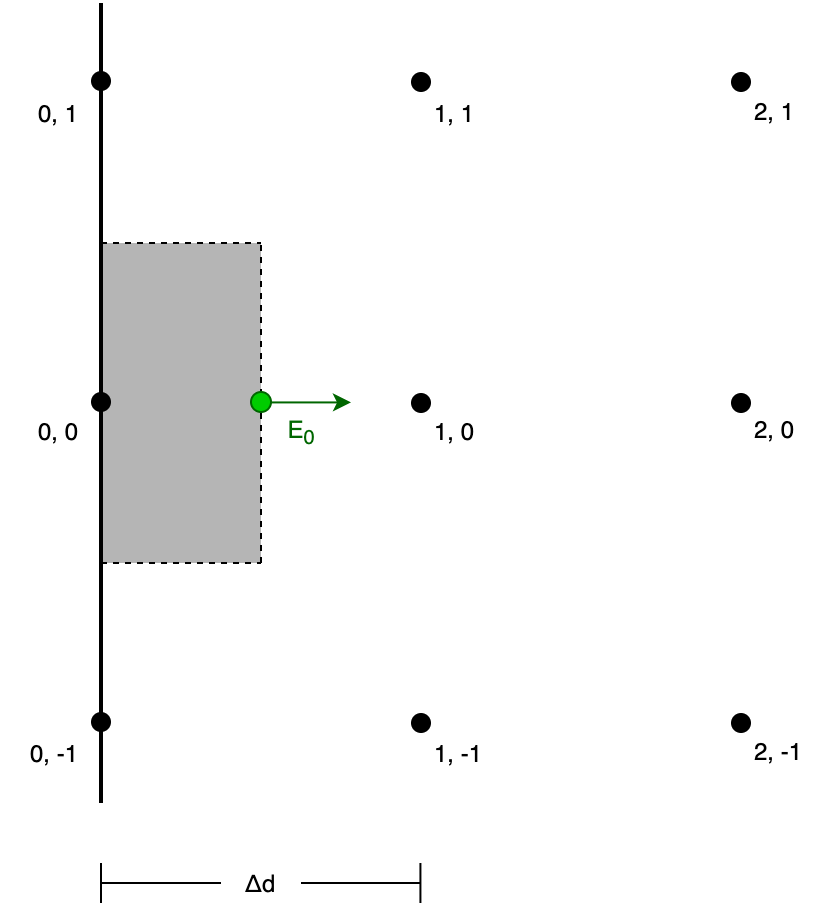
\includegraphics[width=0.6\linewidth]{xoopic/figures/circuit_general_case.png}
	\caption{Illustration of a circuit boundary along a fixed grid.}
	\label{fig:circuit_general_case}
\end{figure} 

The potential at each grid point that intersects the boundary is first taken, then these values are averaged to give the potential of the overall Circuit boundary. For a given point along the boundary, the potential can be computed using Gauss's law. 

The expression for a Gaussian pillbox (shown by the dashed line in figure \ref{fig:circuit_general_case}) is:
\begin{equation}
	\oint_S E \cdot dS = \frac{Q}{\varepsilon_0}
	\label{eq:gauss_law}
\end{equation}
where $Q$ is the charge enclosed by said pillbox. This charge can be expressed as a sum of the volume charge within the pillbox and the surface charge at the boundary:
\begin{equation}
	Q = \oint_V \rho \cdot dV + \oint_S \sigma \cdot dS
	\label{eq:pillbox_charge}
\end{equation}

Combining equations \ref{eq:gauss_law} and \ref{eq:pillbox_charge}, then integrating over their respective areas and volumes results in the expression:
\begin{equation}
	E \cdot A_1 = \frac{1}{\varepsilon_0}(\rho \cdot V + \sigma \cdot A_2)
	\label{eq:gauss_pillbox}
\end{equation}

Note that there are two different areas produced: one related to the surface charge density along the boundary, $A_2$; and one related to electric field out of the pillbox, $A_1$. The values of these terms depend on the geometry used.

The electric field can be expressed in terms of the potential difference:
\begin{equation}
	E = - \nabla \phi
\end{equation}
Thus, the forward-difference method can be used to determine the electric field of the pillbox seen in figure \ref{eq:pillbox_charge}. 
\begin{equation}
	\frac{\phi_0 - \phi_1}{\Delta d} \cdot A_1 = \frac{1}{\varepsilon_0}(\rho \cdot V + \sigma \cdot A_2)
	\label{eq:potential_pillbox}
\end{equation}
An additional note regarding equation \ref{eq:potential_pillbox}, the term $\Delta d$ denotes the distance between the grid points. Similarly to the area and volume terms, this value depends on the geometry used.

As explained in chapter 3, the volume charge densities of particles within PIC simulations are discretised onto the grid using bilinear interpolation. This means the the volume charge of the pillbox is known at the at the grid. Therefore, the only unknown term on the RHS of equation \ref{eq:potential_pillbox} is the surface charge density.

This can be determined using Kirchoff's current law in the circuit shown in figure \ref{fig:circuit}:
\begin{equation}
	\frac{d \sigma}{dt} = J_{cond} + J_{conv}
	\label{eq:kirchoff_current_law}
\end{equation}

Equation \ref{eq:kirchoff_current_law} can be expressed numerically using the backwards-difference method. Additionally, the conduction and convection current density can expressed in terms of their charges, eliminating the $dt$ terms on both sides.
\begin{equation}
	\sigma^t - \sigma^{t - \Delta t} = \frac{1}{A_2} \left(Q^t - Q^{t - \Delta t} + Q_{conv} \right)
	\label{eq:almost_final_surface charge}
\end{equation}
The variables $\sigma^{t - \Delta t}$ and $Q^{t - \Delta t}$ represent quantities determined in the previous time step, thus should be known. Supposing it is the start of the simulation where $t = 0$, they can be simply initialised to zero. $Q_{conv}$ represents the charge deposited onto the boundary by particles since the previous time step. Hence the only  unknown term on the RHS of equation is the conduction charge at the current time step, $Q^t$.

This conduction charge can be determined using Kirchoff's voltage law (also expressed in equation \ref{eq:circuit_equation}, though in a slightly different form):
\begin{equation}
	\phi_0 = V_s - \frac{dQ}{dt} \cdot R_s
	\label{eq:kirchoff_voltage_law}
\end{equation}

The derivative term can again be solved numerically using the backwards-difference. However unlike the other equations, a second order difference is used here to provide a better approximation of the charge. This second order backwards-difference is given as:
\begin{equation}
	\frac{dQ}{dt} = \frac{3Q^t - 4Q^{t - \Delta t} + Q^{t - 2\Delta t}}{2 \Delta t}
	\label{eq:second_order_backwards_difference}
\end{equation}

Combining equations \ref{eq:kirchoff_voltage_law} and \ref{eq:second_order_backwards_difference} provides a new expression for the  conduction charge, $Q^t$:
\begin{equation}
	Q^t = \frac{V_s - \phi_0 - (\alpha_1 Q^{t - \Delta t} + \alpha_2 Q^{t - 2\Delta t})}{\alpha_0}
	\label{eq:conduction_charge}
\end{equation}
where $\alpha_0 = \frac{3}{2}\frac{R_s}{\Delta t}$,  $\alpha_1 = 2\frac{R_s}{\Delta t}$, and  $\alpha_2 = \frac{1}{2}\frac{R_s}{\Delta t}$ are constants to simply the expression. 

Using equation \ref{eq:conduction_charge}, a new surface charge density expression can be determined:
\begin{equation}
	\sigma^t - \sigma^{t - \Delta t} = \frac{1}{A_2} \left(\frac{V_s - \phi_0 - (\alpha_1 Q^{t - \Delta t} + \alpha_2 Q^{t - 2\Delta t})}{\alpha_0} - Q^{t - \Delta t} + Q_{conv} \right)
	\label{eq:final_surface_charge}
\end{equation}

This in turn can be combined with equation \ref{eq:potential_pillbox} from Gauss's law to give the expression:
\begin{equation}
	\frac{\phi_0 - \phi_1}{\Delta d} \cdot A_1 + \frac{\phi_0}{\alpha_0 \  \varepsilon_0} = \frac{1}{\varepsilon_0} \left(\rho \cdot V + \sigma^{t - \Delta t} \cdot A_2 + \left(\frac{V_s - K^t}{\alpha_0} - Q^{t - \Delta t} + Q_{conv} \right) \right)
	\label{eq:almost_final_circuit_equation}
\end{equation}
where $K^t = \alpha_1 Q^{t - \Delta t} + \alpha_2 Q^{t - 2\Delta t}$. Note, that the unknown terms ($\phi_0$ and $\phi_1$) have been rearranged to the  LHS of the equation.

Typically, the coefficients in equation \ref{eq:almost_final_circuit_equation} can then be fed into the field solver to determine the potential of all grid points. However in XOOPIC, the grid potentials of each boundary within the simulation are individually computed before the simulation begins. Then at each time step, the overall potential is determined by summing the predetermined potential induced by the individual boundaries via superposition, and adding the potential due to space charges (from the particles). This approach does not necessarily speed up the computation of the field solver, however it does decouple the boundary code  from the field solver code; making it easier to implement new boundaries.

Because of this pre-computation, equation \ref{eq:almost_final_circuit_equation} can be simplified by specifying $\phi_1 = c_1 \phi_0$, where $c_1$ is the ratio of $\phi_1/\phi_0$. Hence, the general solution for a circuit boundary can be given as:
\begin{equation}
	\phi_0 \left((1 - c_1)A_1 + \frac{\Delta d}{\alpha_0 \ \varepsilon_0} \right) = \frac{\Delta d}{\varepsilon_0} \left(\rho \cdot V + \sigma^{t - \Delta t} \cdot A_2 + \left(\frac{V_s - K^t}{\alpha_0} - Q^{t - \Delta t} + Q_{conv} \right) \right)
	\label{eq:final_circuit_equation}
\end{equation}


\subsubsection{Cartesian Geometry}

There are two possible orientations for the Circuit boundary for the cartesian geometry: along (or parallel to) the $x$-axis, or along the $y$-axis. Therefore, the variables seen in the left most column of table \ref{tb:variables_cartesian_geometry} should be replaced by their values in the given orientation of the Circuit boundary.

\begin{table}[h!]
	\caption{Circuit boundary variables for cartesian geometry.}
	\vspace{5 pt}
	\centering
	\begin{tabular}{c c c}
		Variables  & Along $x$-axis      		   & Along $y$-axis       \\
		\hline 
		$\Delta d$ & $\Delta y$           		   & $\Delta x$           \\
		$A_1$      & $\Delta x \Delta z$  		   & $\Delta y \Delta z$  \\
		$A_2$      & $\Delta x \Delta z$           & $\Delta y \Delta z$  \\
		$V$        & $\Delta x \Delta y \Delta z$  & $\Delta y \Delta y  \Delta z$
	\end{tabular}
	\label{tb:variables_cartesian_geometry}
\end{table}

When operating in the cartesian coordinate system, the two area terms $A_1$ and $A_2$ are identical irregardless of the orientation. 

\subsubsection{Cylindrical Geometry}

The two possible orientations for a cylindrical geometry are: along the r-axis, or along the z-axis. However, unlike the cartesian geometry where $A_1$ always equals $A_2$ for both orientation, this only holds for the case where the Circuit boundary is along the r-axis. For the case along the z-axis, $A_1$ and $A_2$ are distinct. 

The terms for a given orientation of the Circuit boundary in cylindrical geometry can be seen in table \ref{tb:variables_cylindrical_geometry}.

\begin{table}[h!]
	\caption{Circuit boundary variables for cylindrical geometry.}
	\vspace{5 pt}
	\centering
	\begin{tabular}{c c c}
		Variables  & Along $z$-axis      		   & Along $r$-axis       \\
		\hline 
		$\Delta d$        & $\Delta r$           		   & $\Delta z$           \\
		$A_1$      & $2\pi r_{i + 0.5\Delta r} \Delta z$  		   & $\pi (r_{j + 0.5\Delta r}^2 - r_{j - 0.5\Delta r}^2)$  \\
		$A_2$      & $2\pi r_i \Delta z$           & $\pi (r_{j + 0.5\Delta r}^2 - r_{j - 0.5\Delta r}^2)$  \\
		$V$        & $\pi (r_{i + 0.5\Delta r}^2 - r_i^2)\Delta z$  & $\frac{1}{2} \pi (r_{j + 0.5\Delta r}^2 - r_{j - 0.5\Delta r}^2)\Delta z$
	\end{tabular}
	\label{tb:variables_cylindrical_geometry}
\end{table}

\subsection{Validation}

The validation for the Circuit boundary was done in two parts. The first was a test case without particles, which was then followed by one with particles. The former was used to evaluate the accuracy of the boundary calculations itself, without the computation from particles (i.e. the discretisation of the volume charge densities or the count of the number of particles colliding with the boundary). The latter was to test the operation of the boundary in a simulation scenario, which almost always has particles.

For both test cases, only simulation of a device in cartesian geometry is shown for the sake of brevity and the fact that the solution to the potential of the circuit boundary is highly dependant on the geometry (as discussed in the previous subsection). 

\subsubsection{Test Case without Particles}

\begin{figure}[h!]
	\centering
	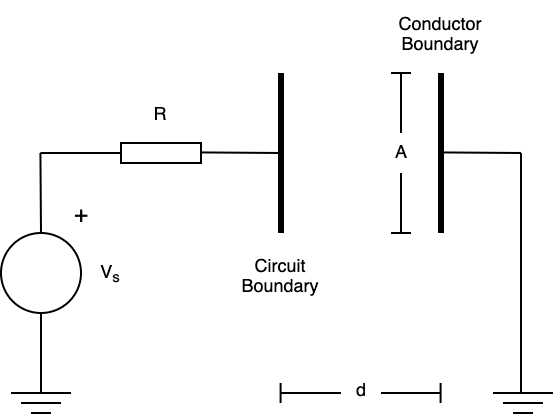
\includegraphics[width=0.59\linewidth]{xoopic/figures/circuit_test.png}
	\caption{Illustration of test case for Circuit boundary without particles.}
	\label{fig:circuit_test}
\end{figure} 

An illustration of the device being simulated can be seen in figure \ref{fig:circuit_test}, where the Circuit boundary was placed along the $y$-axis at the left-most wall and a grounded \textit{Conductor} boundary placed along the right-most wall. This device, without any particles, essentially behaves as a capacitor with a capacitance given by $C = \frac{\varepsilon_0 A}{d}$. The parameters for this test case can be found in table \ref{tb:test_1}

\begin{table}[h!]
	\caption{Parameters for test case of Circuit boundary without particles.}
	\vspace{5 pt}
	\centering
	\begin{tabular}{c c}
		Parameters  & Values 	    \\
		\hline 
		$V_s$       & 1000 V        \\
		$R$         & 1000 $\Omega$ \\
		$A$         & 0.05 m$^2$    \\
		$d$         & 0.05 m	    \\
		$C$			& 8.85 pF
	\end{tabular}
	\label{tb:test_1}
\end{table}

Thus, this simulation models the charging of a capacitor in an $RC$ circuit, which can be expressed as:
\begin{equation}
	V_c = V_s(1 - e^{-t/\tau})
	\label{eq:rc_circuit}
\end{equation}
where the time constant is $\tau = RC$. 

\begin{figure}[h!]
	\centering
	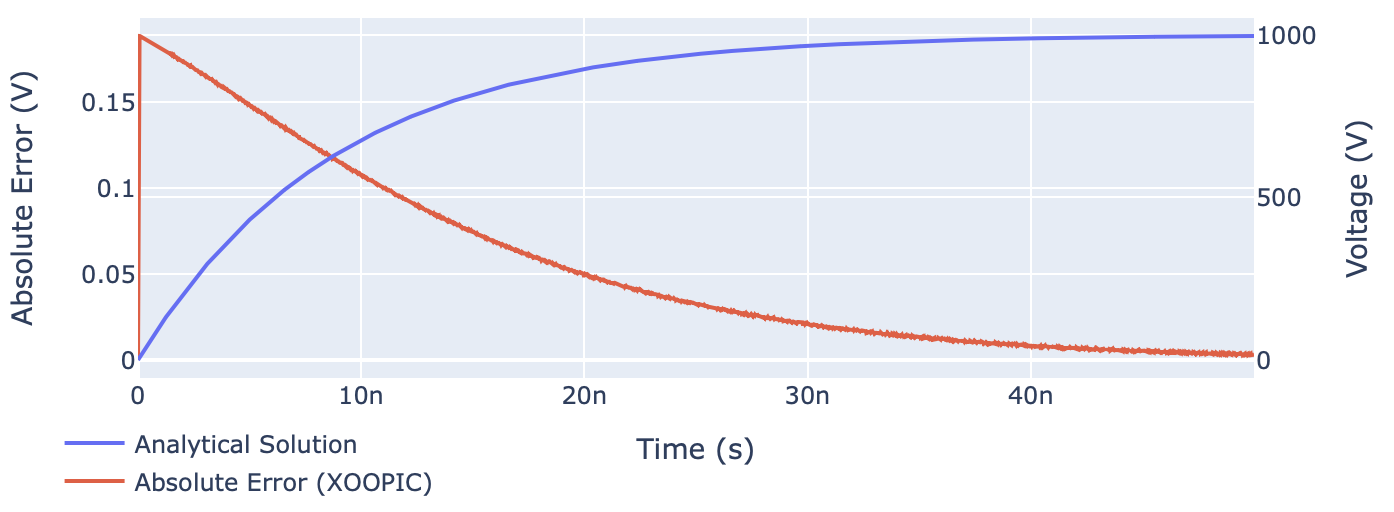
\includegraphics[width=\linewidth]{xoopic/figures/test_1_error.png}
	\caption{Comparison between the analytical solution and XOOPIC, where $\Delta t = 10$ ps.}
	\label{fig:test_1_error}
\end{figure} 

For the simulated device, $C = 8.85$ pF and $\tau = 8.85$ ns. From this, an analytical solution can be determined, with the RC curve shown in figure \ref{fig:test_1_error}. For the XOOPIC simulation, a run was performed from $t=0$ to $t=50$ ns (approximately 5 time constants), with a time step of $\Delta t = 10$ ps. The resulting RC curve overlapped the the one produced by the analytical solution, hence only the absolute error is shown. 

\begin{figure}[h!]
	\centering
	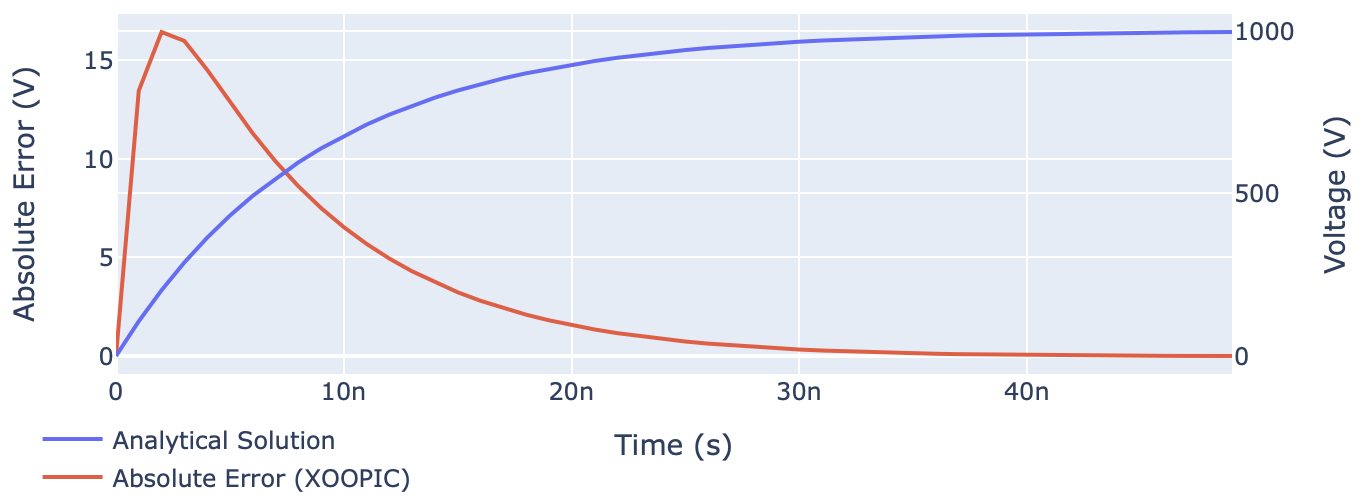
\includegraphics[width=\linewidth]{xoopic/figures/test_1_bigger_error.png}
	\caption{Comparison between the analytical solution and XOOPIC, where $\Delta t = 1$ ns.}
	\label{fig:test_1_bigger_error}
\end{figure}

\begin{figure}[h!]
	\centering
	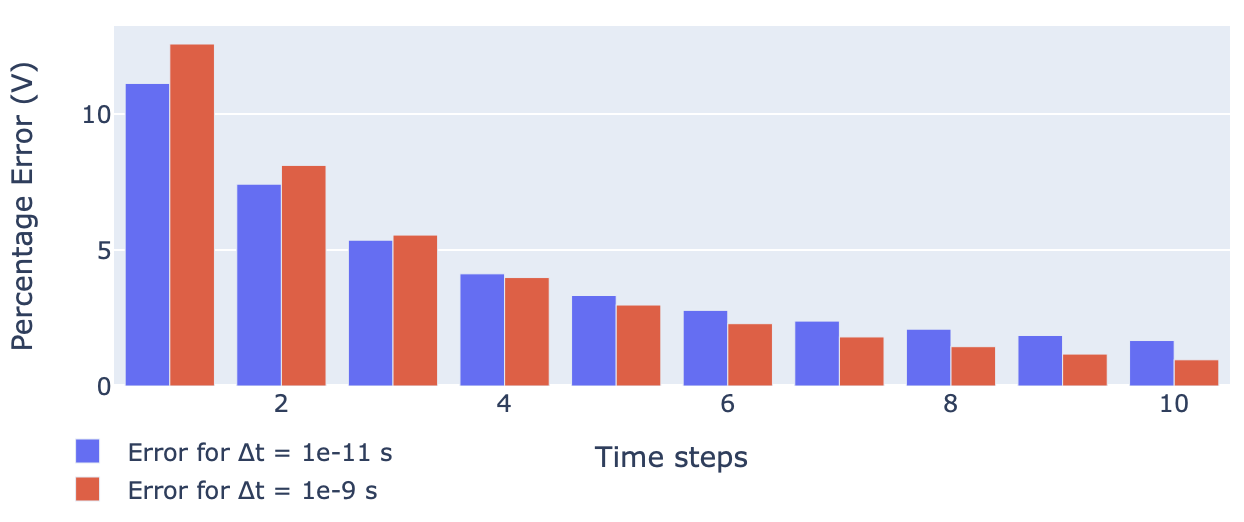
\includegraphics[width=\linewidth]{xoopic/figures/test_1_error_comparison.png}
	\caption{Comparison of the error from XOOPIC when $\Delta t = 10$ ps and $\Delta t = 1$ ns.}
	\label{fig:test_1_error_comparison}
\end{figure} 

This error seen is a convergence error, which is due to the conduction charge values requiring a finite number of iterations before they converge to the true value. To illustrate this, the same simulation is run with a larger time step of  $\Delta t = 1$ ns (100 times that of the original simulation). These results can be seen in figure \ref{fig:test_1_bigger_error}. Notice that there is a significantly larger absolute error (nearly 100 times greater). However when observing the percentage error, seen in figure \ref{fig:test_1_error_comparison}, the differences are quite comparable. Therefore, so long as the time step used is sufficiently small (to ensure a small absolute error), the simulations can be said to be accurate enough.

\subsubsection{Test Case with Particles}

Generating a simplified test case to only asses the impact of particles on the Circuit boundary was slightly more challenging. The simulated circuit for this test case can be seen in figure \ref{fig:circuit_test_2}. As for the parameters used, they can be found in table \ref{tb:test_2}. 

\begin{figure}[h!]
	\centering
	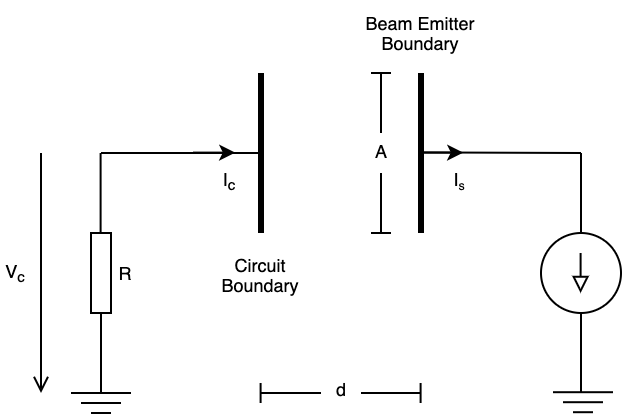
\includegraphics[width=0.65\linewidth]{xoopic/figures/circuit_test_2.png}
	\caption{Illustration of test case for Circuit boundary without particles.}
	\label{fig:circuit_test_2}
\end{figure} 

\begin{table}[h!]
	\caption{Parameters for test case of Circuit boundary with particles.}
	\vspace{5 pt}
	\centering
	\begin{tabular}{c c}
		Parameters  & Values 	    			\\
		\hline 
		$V_s$       & 0 V      			        \\
		$I_s$		& 1 A						\\
		$R$         & 1000 $\Omega$ 			\\
		$A$         & $5 \times 10^{-4}$ m$^2$  \\
		$d$         & $5 \times 10^{-4}$ m      \\
		$C$			& 8.85 pF					\\
		$v_{d, x}$	& 1000 eV					\\
		$v_{d, y}$	& 0 eV
	\end{tabular}
	\label{tb:test_2}
\end{table}


Notice that the grounded Conductor boundary was replaced with a \textit{Beam Emitter} boundary. The Beam Emitter is similar to the Current Source boundary, wherein a steady supply of charge is supplied to the boundary. However, unlike the Current Source which simply deposits the charge at the boundary (which in turn generates a potential), the Beam Emitter releases this charge into the simulation domain in the form of particles. This steady source of particles is what enabled the evaluation of this test case. The particles emitted out of the Beam Emitter (i.e. towards the LHS) in this case were electrons, hence why source current $I_s$ is shown in the opposite direction. To ensure no particle losses, collisions by the MCC were turned off, the simulated device was set to a vacuum, and the drift velocity of the particles along the $y$-axis, $v_{d, y}$ was set to 0 eV. 

As for the Circuit boundary itself, the source voltage $V_s$ was grounded, implying that the potential of the boundary is solely given by the current through the resistor, $I_c$. Additionally, because the source current must be equal to the circuit current (as there were no losses) and one end of the resistor was grounded, the potential at the Circuit boundary has to be negative.

The analytical solution for this test case is given by the conduction current from electrons colliding with the Circuit boundary, and the displacement current across the capacitor. The conduction current is merely a step from 0 A to the $-1$ A specified by the source current. It is negative because the current is leaving the boundary. The time at which this step occurs is given by the time taken for the electrons to travel across the device. As the drift velocity of the electrons along the direction of the $x$-axis was set to $v_{d, x} = 1000$ eV, thus its true velocity can be determined using the equation for kinetic energy:
\begin{equation}
	E_{ke} = \frac{1}{2}mv^2
\end{equation}

where 1 eV = $1.6 \times 10^-{19}$ J. 

This resulted in a velocity of approximately $1.87 \times 10^7 \ ms^{-1}$, hence it crossed the length of the device in roughly 30 ps. Thus this is when the step in conduction current should occur.

As for the displacement current, this is given by:
\begin{equation}
	I_{disp} = C\ \frac{dV}{dt}
\end{equation}

Combining this with the analytical solution of the RC circuit in equation \ref{eq:rc_circuit}, gives the displacement current of:
\begin{equation}
	I_{disp} = \frac{V_{ss}}{R}e^{-\frac{t}{\tau}}
\end{equation}
where $V_{ss}$ is the potential difference across the capacitor when it reaches a steady state, which is given as $V_{ss} = I_s R$. The displacement current is in opposite the opposite direction to the conduction current, hence in this case it is positive. Similiarly to the conduction current, the displacement current at the surface of the Circuit boundary would only occur after the electrons collide with the boundary itself. 

The overall potential is obtained by combining the contributions of the conduction and displacement currents with the resistance of the circuit. This is expressed in the equation below, and is illustrated in figure \ref{fig:test_2_error}.
\begin{equation}
	V_c = 
	\begin{cases}
		0 								  &\text{t $< 30$ ps} \\
		I_s R\ (e^{-\frac{t}{\tau}} - 1) &\text{t $>= 30$ ps}
	\end{cases}
\end{equation}

For the simulation, a similar overall device geometry was used to that of the the previous test, however the gap distance $d$ was decreased to minimise the time required for the electrons to collide with the boundary. This meant that the area of the boundary plates $A$ also had to be decreased to ensure that the capacitance, and by extension the time constant, remained the same. Again, the simulations were run from $t=0$ to $t=50$ ns, with a time step of $\Delta t = 10$ ps. Figure \ref{fig:test_2_error} also shows the absolute error of the Circuit boundary of the simulation as apposed to that of the analytical solution. The error observed is much larger with a maximum error of approximately 26 V; quite a significant error. However, at the time of writing this report, the origin of this error is still unknown.

\begin{figure}[h!]
	\centering
	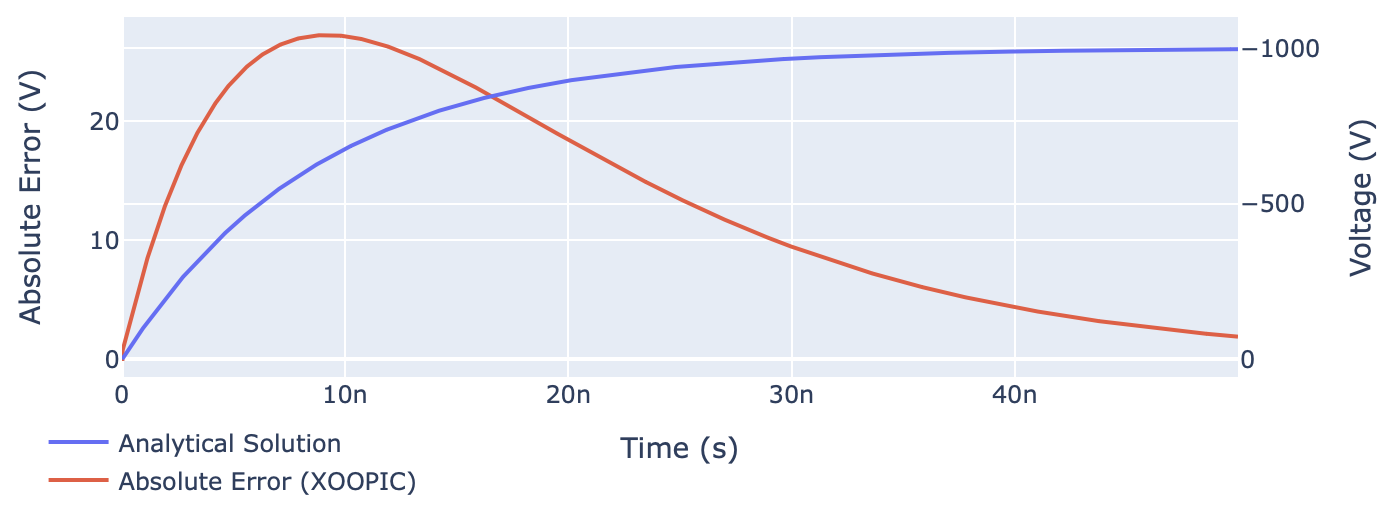
\includegraphics[width=\linewidth]{xoopic/figures/test_2_error.png}
	\caption{Illustration of test case for Circuit boundary without particles.}
	\label{fig:test_2_error}
\end{figure} 

\subsection{Future Work}

Aside from the Circuit boundary simulating a more accurate “real world” voltage source, it can possibly be used in model more complicated circuit networks. This is because, Thevenin's theorem dictates that any linear circuit network can be represented by an equivalent circuit that contains a voltage source with a series impedance (which is a resistance in this case). 

Nonetheless, most circuits also contain some amount of capacitance and/or inductance. Hence, it could potentially be beneficial to add a series inductor and capacitor to the Circuit boundary in addition to the existing resistor. To achieve this, the the RHS of Kirchoff's voltage law, equation \ref{eq:kirchoff_voltage_law}, needs to be modified to include the potential due to the inductor, $V = \frac{d^2Q}{dt^2} L$, and the potential due to a capacitor, $V = \frac{Q}{C}$. This new equation can be rearranged to solve for the current conduction charge. From there, the same process can be applied to determine the potential of the Circuit boundary.